\documentclass[10pt,twocolumn]{article}
\usepackage[margin=0.8in,top=0.9in,bottom=0.9in]{geometry}
\usepackage{amsmath,amssymb,booktabs,graphicx,microtype,xcolor,url}
\usepackage[numbers,sort&compress]{natbib}
\usepackage[hidelinks]{hyperref}
\usepackage{caption}
\captionsetup{font=small,labelfont=bf}
\renewcommand{\topfraction}{0.95}\renewcommand{\textfraction}{0.05}\renewcommand{\floatpagefraction}{0.75}
\newcommand{\nModels}{4}
\newcommand{\nDatasets}{7}
\newcommand{\Jbest}{0.476}
\newcommand{\JbootLo}{0.16}
\newcommand{\JbootHi}{0.50}
\newcommand{\JEm}{0.362}
\newcommand{\JRc}{0.429}
\newcommand{\JUni}{0.429}
\newcommand{\JFone}{0.459}
\newcommand{\pairTauBest}{0.136}
\newcommand{\pairTauEm}{0.045}
\newcommand{\dispBest}{2.06}
\newcommand{\dispEm}{2.10}
\newcommand{\tauNative}{0.67}
\newcommand{\tauEmPool}{0.33}
\newcommand{\topOne}{gpt-5.5}
\newcommand{\topTwo}{claude-opus-5}
\newcommand{\topThree}{claude-sonnet-5}
\newcommand{\medianJ}{0.381}
\newcommand{\minJ}{0.180}
\newcommand{\nAboveEm}{65}
\newcommand{\lodoMean}{0.35}
\newcommand{\lodoFullMean}{0.40}
\newcommand{\weightsStr}{em 0.05, num\_tol 0.25, num\_decay 0.05, tok\_prec 0.05, tok\_rec 0.15, edit\_sim 0.15, rouge\_l 0.25, jaccard 0.05}

\title{\textbf{One Score Across Data-Matching Benchmarks:\\Random-Search Weight Calibration and Rank Pooling for LLM Evaluation}}
\author{Data Matchmaker Benchmark v2 \\ \small Green-agent evaluator for the AgentBeats A2A platform}
\date{}
\begin{document}
\maketitle
\begin{abstract}
Benchmarks for data-matching and financial table reasoning each ship their own metric, so per-dataset scores of a language model cannot be added up into one number, and per-dataset leaderboards disagree. We propose a simple, fully reproducible recipe for a common score: (i) a composite answer metric $S=\sum_k w_k m_k$ over nine component metrics; (ii) a random search over 100 weight combinations drawn from a simplex grid, scored by how well each dataset's model ranking agrees with the pooled ranking of all datasets (mean Kendall $\tau$ to the Borda ensemble); (iii) an ensemble leaderboard that pools per-dataset rankings with Borda, Copeland, Kemeny--Young and reciprocal-rank fusion, with bootstrap confidence intervals over items. On seven diverse, widely used datasets from the benchmark's original catalogue (OfficeQA, FinQA, TAT-QA, TabFact, FinanceBench, FeTaQA, WikiTableQuestions) and \nModels{} commercial models, the best combination raises the agreement objective from $\JEm$ (exact match) and $\JRc$ (the previous hand-set rubric) to $\Jbest$, but the bootstrap interval $[\JbootLo, \JbootHi]$ shows that with four closely matched models and 40 items per dataset the per-dataset rankings are too noisy for any weighting to make them agree strongly; we report this limitation, the leave-one-dataset-out transfer, and the pooled leaderboard with its uncertainty. We also describe, but do not adopt, Kullback--Leibler and Jensen--Shannon divergence between score distributions as an extension of the objective.
\end{abstract}

\section{Introduction}
The Data Matchmaker green agent \cite{a2a2025,tpcdi2014} evaluates purple agents on a catalogue of data-matching tasks: Treasury bulletins (OfficeQA \cite{officeqa2026}), SEC filings with tables and text (FinQA \cite{chen2021finqa}, TAT-QA \cite{zhu2021tatqa}, FinanceBench \cite{islam2023financebench}), Wikipedia tables (TabFact \cite{chen2020tabfact}, FeTaQA \cite{nan2022fetaqa}, WikiTableQuestions \cite{pasupat2015wtq}). The catalogue was chosen for diversity (documents, hybrid table+text, pure tables; numeric, span, boolean and free-form answers) and for importance (each is a standard, heavily cited benchmark). Each dataset, however, defines its own metric, and the original judge combined them with a hand-set rubric. The goal of this paper is an \emph{aggregate common score}: one weighting of component metrics under which a model's score means the same thing on every dataset, so that per-dataset results can be pooled into a single leaderboard.

Our contributions are (1) a random search over 100 grid combinations of component weights with a ranking-consistency objective (\S\ref{sec:method}); (2) a pooled leaderboard under several rank-aggregation rules with bootstrap uncertainty (\S\ref{sec:pool}); (3) an honest analysis of how much such calibration can achieve with seven models and 40 items per dataset (\S\ref{sec:results}); and (4) a documented extension using KL/JS divergence between score distributions, provided as a standalone file (\S\ref{sec:ext}).

\section{Related work}
Rank aggregation for benchmarks is classical \cite{dwork2001rank,young1978consistent,cormack2009rrf} and has been advocated for NLP leaderboards \cite{colombo2022ranking}; HELM \cite{liang2022helm} and BIG-bench \cite{srivastava2023bigbench} pool scenarios by mean win rate or mean rank. Metric meta-evaluation in machine translation \cite{mathur2020tangled,freitag2021experts} warns that metric choice changes rankings; we make the choice explicit and search over it. Component metrics follow SQuAD EM/F1 \cite{rajpurkar2016squad} and ROUGE-L \cite{lin2004rouge}; divergences follow \cite{lin1991divergence}.

\section{Method}\label{sec:method}
\paragraph{Composite metric.} For a prediction $p$ and gold $g$ we compute nine component metrics in $[0,1]$: exact match (after normalisation, with unit/percent-aware numbers, list golds and gold aliases such as \texttt{14\%} $\equiv$ \texttt{0.14464}), numeric tolerance ($\le 1\%$ relative error), numeric decay $e^{-2.5\,\mathrm{RE}}$, token precision, recall and F1, normalised edit similarity, ROUGE-L and Jaccard. The composite is $S(p,g)=\sum_{k=1}^{9} w_k m_k(p,g)$ with one global weight vector $w$ on the probability simplex.
\paragraph{Objective.} Let $\bar S_{m,d}(w)$ be model $m$'s mean composite on dataset $d$, $r_d(w)$ the ranking of models on $d$ and $R(w)$ the Borda ensemble of the $r_d$. We maximise
\begin{equation}
J(w)=\frac{1}{|\mathcal D|}\sum_{d}\tau\big(r_d(w),R(w)\big),
\end{equation}
the mean Kendall $\tau$ between each dataset's ranking and the pooled ranking: weights under which datasets ``vote alike''. We also report the mean pairwise $\tau$ between datasets and a scale-dispersion statistic (how much a model's difficulty-centred score moves between datasets, relative to the spread between models).
\paragraph{Random search on the grid.} We draw 100 distinct weight vectors by sampling $\mathrm{Dirichlet}(\mathbf 1)$ points and snapping them to the simplex grid with step $0.05$ (seed fixed), evaluate $J$ for each, rank them, and bootstrap $J$ (200 item resamples) for the top five, the median and the worst. Fixed baselines (EM only, F1 only, numeric tolerance only, uniform, the v1 rubric $R_{custom}=0.35F_1+0.35e^{-2.5\mathrm{MRE}}+0.15P+0.15R$) are evaluated under the same objective. Leave-one-dataset-out (LODO) re-selects the best combination without each dataset and measures the held-out dataset's agreement with the pooled ranking of the rest.

\section{Pooling}\label{sec:pool}
Given $\bar S_{m,d}$ under the calibrated weights, the \emph{common score} is the mean over datasets (and, difficulty-adjusted, the mean of per-dataset $z$-scores). The pooled ranking is computed with mean score, mean $z$, mean rank, Borda, Copeland, Kemeny--Young (exact, 7 systems) and reciprocal-rank fusion; uncertainty comes from resampling items within every dataset 1{,}000 times and recomputing the Borda consensus.

\section{Setup}
Seven datasets from the original catalogue, 40 stratified items each (numeric / boolean / text / free-form golds; OfficeQA is closed-book because its corpus is gated), and \nModels{} industry-standard models, the flagship and standard tier of two providers with usable API access at the time of writing (OpenAI GPT-5.5 and GPT-5.4-mini; Anthropic Claude Opus 5 and Sonnet 5), queried once per item with one prompt that requests a \texttt{FINAL ANSWER:} line. Predictions are cached; the search itself costs seconds. The model catalogue (\texttt{config/models.toml}) also lists Gemini 3.1 Pro / 3.8 Flash, Grok-4, Llama-3.3-70B, DeepSeek-V3/R1, Qwen-2.5-72B and Mistral Large; each runs automatically once its API key is available (Gemini's key was quota-exhausted and xAI's had no credits during this study).

\section{Results}\label{sec:results}
\paragraph{Random search.} Table~\ref{tab:rs} lists the ten best combinations and Figure~\ref{fig:rs} the full distribution. The best vector (\weightsStr) reaches $J=\Jbest$; the median combination reaches $\medianJ$ and the worst $\minJ$. Only \nAboveEm{} of the 100 combinations beat EM-only ($J=\JEm$); the v1 rubric ($\JRc$) and the uniform composite ($\JUni$) are near the bottom (Table~\ref{tab:baselines}). The top vectors share a pattern: numeric tolerance and ROUGE-L carry the largest shares, with recall and edit similarity next and almost no exact match, i.e.\ a firm numeric check plus graded credit for partially correct spans.
\paragraph{How much is signal.} The bootstrap interval of the best $J$ is $[\JbootLo,\JbootHi]$, which contains EM-only and most of the top ten. The mean pairwise $\tau$ between datasets is $\pairTauBest$ for the best weights and $\pairTauEm$ for EM: the datasets barely agree on the ordering of these seven models under \emph{any} weighting, because the four models are close in ability, TabFact and TAT-QA are near ceiling, OfficeQA is at floor and 40 items leave many ties. LODO (Table~\ref{tab:lodo}) confirms this: the held-out agreement under weights selected without the dataset averages $\lodoMean$ versus $\lodoFullMean$ with the full-data weights, with sign flips on TabFact and TAT-QA. The calibration therefore improves the objective, but the improvement is within noise at this sample size; more items per dataset and more, and more diverse, models are the direct remedy.
\paragraph{Pooled leaderboard.} Table~\ref{tab:leaderboard} and Figure~\ref{fig:lb} give the common score and pooled ranks. \topOne{} leads under every rule, followed by \topTwo{} and \topThree{}; below rank 1 the bootstrap intervals overlap. The rules agree with each other (Table~\ref{tab:rules}); the pooled ranking agrees with the native-metric pooled ranking at $\tau=\tauNative$ and with the EM-only pooled ranking at $\tauEmPool$. Table~\ref{tab:dsagree} shows which datasets vote with the consensus.

\begin{figure*}[t]\centering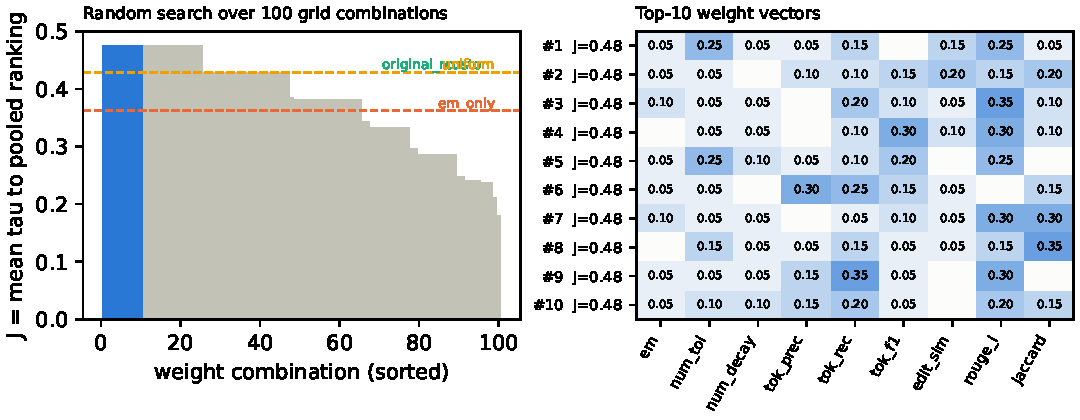
\includegraphics[width=0.9\textwidth]{../output/rs/fig_random_search.pdf}
\caption{Left: $J$ for the 100 random grid combinations (blue = top 10) with baselines as dashed lines. Right: the top-10 weight vectors.}\label{fig:rs}\end{figure*}
\begin{figure*}[t]\centering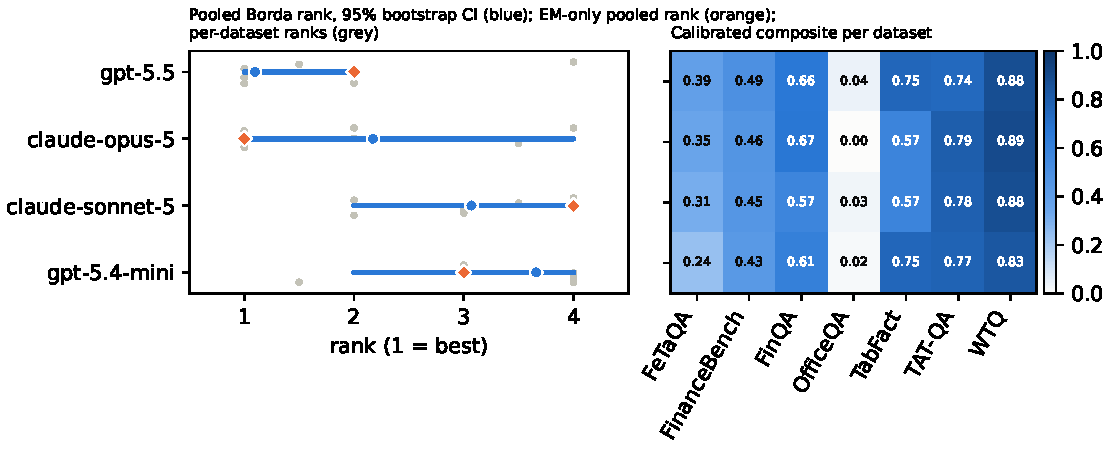
\includegraphics[width=0.95\textwidth]{../output/rs/fig_leaderboard.pdf}
\caption{Pooled Borda rank with 95\% bootstrap CI, EM-only pooled rank, per-dataset ranks (left) and per-dataset calibrated scores (right).}\label{fig:lb}\end{figure*}
\begin{table*}[t]
\centering
\footnotesize
\caption{Top-10 of the 100 random weight combinations (grid step 0.05). $J$ = mean Kendall $\tau$ between each dataset's model ranking and the pooled Borda ranking.}
\label{tab:rs}
\resizebox{\textwidth}{!}{%
\begin{tabular}{lrrrrrrrrrrrrr}
\toprule
\# & $J$ & boot 95\% CI & pairwise $\tau$ & disp. & em & num\_tol & num\_decay & tok\_prec & tok\_rec & tok\_f1 & edit\_sim & rouge\_l & jaccard \\
\midrule
1 & 0.476 & [0.16, 0.50] & 0.136 & 2.06 & 0.05 & 0.25 & 0.05 & 0.05 & 0.15 & -- & 0.15 & 0.25 & 0.05 \\
2 & 0.476 & [0.16, 0.50] & 0.136 & 1.95 & 0.05 & 0.05 & -- & 0.10 & 0.10 & 0.15 & 0.20 & 0.15 & 0.20 \\
3 & 0.476 & [0.17, 0.50] & 0.136 & 1.97 & 0.10 & 0.05 & 0.05 & -- & 0.20 & 0.10 & 0.05 & 0.35 & 0.10 \\
4 & 0.476 & [0.16, 0.50] & 0.136 & 1.95 & -- & 0.05 & 0.05 & -- & 0.10 & 0.30 & 0.10 & 0.30 & 0.10 \\
5 & 0.476 & [0.16, 0.50] & 0.136 & 2.04 & 0.05 & 0.25 & 0.10 & 0.05 & 0.10 & 0.20 & -- & 0.25 & -- \\
6 & 0.476 & -- & 0.136 & 1.88 & 0.05 & 0.05 & -- & 0.30 & 0.25 & 0.15 & 0.05 & -- & 0.15 \\
7 & 0.476 & -- & 0.136 & 1.98 & 0.10 & 0.05 & 0.05 & -- & 0.05 & 0.10 & 0.05 & 0.30 & 0.30 \\
8 & 0.476 & -- & 0.136 & 1.96 & -- & 0.15 & 0.05 & 0.05 & 0.15 & 0.05 & 0.05 & 0.15 & 0.35 \\
9 & 0.476 & -- & 0.136 & 1.92 & 0.05 & 0.05 & 0.05 & 0.15 & 0.35 & 0.05 & -- & 0.30 & -- \\
10 & 0.476 & -- & 0.136 & 2.00 & 0.05 & 0.10 & 0.10 & 0.15 & 0.20 & 0.05 & -- & 0.20 & 0.15 \\
\bottomrule
\end{tabular}
}
\end{table*}
\begin{table}[t]
\centering
\small
\caption{Fixed baselines vs.\ the random-search optimum under the same objective.}
\label{tab:baselines}

\begin{tabular}{lrrr}
\toprule
Weights & $J$ & pairwise $\tau$ & dispersion \\
\midrule
em\_only & 0.362 & 0.045 & 2.10 \\
f1\_only & 0.459 & 0.123 & 1.83 \\
num\_tol\_only & 0.359 & 0.039 & 3.06 \\
original\_rcustom & 0.429 & 0.069 & 2.28 \\
uniform & 0.429 & 0.069 & 2.08 \\
random\_search\_best & 0.476 & 0.136 & 2.06 \\
\bottomrule
\end{tabular}

\end{table}
\begin{table*}[t]
\centering
\footnotesize
\caption{Leave-one-dataset-out: best combination chosen without the held-out dataset, then agreement of the held-out dataset's ranking with the pooled ranking of the rest.}
\label{tab:lodo}

\begin{tabular}{lrrrr}
\toprule
Held-out & $J$ w/o & $\tau$ held-out (LODO w) & $\tau$ held-out (full w) & $L_1$ shift \\
\midrule
FeTaQA & 0.389 & 1.00 & 1.00 & 0.0 \\
FinanceBench & 0.389 & 0.67 & 1.00 & 0.6 \\
FinQA & 0.500 & 0.33 & 0.33 & 0.0 \\
OfficeQA & 0.488 & 0.00 & 0.00 & 0.0 \\
TabFact & 0.609 & -0.22 & -0.22 & 0.0 \\
TAT-QA & 0.556 & 0.00 & 0.00 & 0.0 \\
WTQ & 0.444 & 0.67 & 0.67 & 0.0 \\
\bottomrule
\end{tabular}

\end{table*}
\begin{table*}[t]
\centering
\small
\caption{Per-dataset calibrated composite, common score (mean and difficulty-adjusted $z$-mean) and pooled ranks; CI from 1{,}000 item bootstraps.}
\label{tab:leaderboard}
\resizebox{\textwidth}{!}{%
\begin{tabular}{lrrrrrrrrrrrrrr}
\toprule
Model & FeTaQA & FinanceBench & FinQA & OfficeQA & TabFact & TAT-QA & WTQ & Common & $z$-mean & Borda & Kemeny & RRF & 95\% CI & Native \\
\midrule
gpt-5.5 & 0.39 & 0.49 & 0.66 & 0.04 & 0.75 & 0.74 & 0.88 & 0.564 & +0.57 & 1 & 1 & 1 & [1, 2] & 1 \\
claude-opus-5 & 0.35 & 0.46 & 0.67 & 0.00 & 0.57 & 0.79 & 0.89 & 0.534 & +0.15 & 2 & 2 & 2 & [1, 4] & 3 \\
claude-sonnet-5 & 0.31 & 0.45 & 0.57 & 0.03 & 0.57 & 0.78 & 0.88 & 0.513 & -0.20 & 3 & 3 & 3 & [2, 4] & 2 \\
gpt-5.4-mini & 0.24 & 0.43 & 0.61 & 0.02 & 0.75 & 0.77 & 0.83 & 0.521 & -0.52 & 4 & 4 & 4 & [2, 4] & 4 \\
\bottomrule
\end{tabular}
}
\end{table*}
\begin{table}[t]
\centering
\footnotesize
\caption{Kendall $\tau$ between the consensus rankings produced by different pooling rules.}
\label{tab:rules}

\begin{tabular}{lrrrrrrr}
\toprule
Rule & mean\_score & mean\_z & mean\_rank & borda & copeland & rrf & kemeny \\
\midrule
mean\_score & 1.00 & 0.67 & 0.67 & 0.67 & 0.67 & 0.67 & 0.67 \\
mean\_z & 0.67 & 1.00 & 1.00 & 1.00 & 1.00 & 1.00 & 1.00 \\
mean\_rank & 0.67 & 1.00 & 1.00 & 1.00 & 1.00 & 1.00 & 1.00 \\
borda & 0.67 & 1.00 & 1.00 & 1.00 & 1.00 & 1.00 & 1.00 \\
copeland & 0.67 & 1.00 & 1.00 & 1.00 & 1.00 & 1.00 & 1.00 \\
rrf & 0.67 & 1.00 & 1.00 & 1.00 & 1.00 & 1.00 & 1.00 \\
kemeny & 0.67 & 1.00 & 1.00 & 1.00 & 1.00 & 1.00 & 1.00 \\
\bottomrule
\end{tabular}

\end{table}
\begin{table}[t]
\centering
\small
\caption{Kendall $\tau$ between each dataset's ranking and the pooled Borda ranking under the calibrated weights.}
\label{tab:dsagree}

\begin{tabular}{lrrrrrr}
\toprule
FeTaQA & FinanceBench & FinQA & OfficeQA & TabFact & TAT-QA & WTQ \\
\midrule
1.00 & 1.00 & 0.33 & 0.33 & 0.00 & 0.00 & 0.67 \\
\bottomrule
\end{tabular}

\end{table}

\section{Extension: divergence objectives}\label{sec:ext}
Rankings ignore the score scale. As an extension we describe (file \texttt{extensions/divergence\_extension.py}, with a write-up in \texttt{extensions/DIVERGENCE\_EXTENSION.md}; not used by the pipeline) a term that compares the whole distribution of a model's item scores on two datasets, after removing dataset difficulty, with Jensen--Shannon divergence (bounded, symmetric) and reports symmetric KL and 1-Wasserstein distance alongside. On the cached data, mean $\mathrm{JS}/\ln 2$ across dataset pairs is $0.86$ for EM-only, $0.77$ for the v1 rubric and $0.78$ for the random-search weights: graded weightings give more comparable score profiles than exact match, and the ranking objective alone does not further reduce divergence, which is the case for adding the term. The write-up also explains why divergence cannot be the sole objective: a binary metric that fails uniformly has identical Bernoulli histograms everywhere (EM reaches $\mathrm{JS}\approx 0.005$ between TabFact and TAT-QA for that reason), so a ranking or known-quality anchor term is required.

\section{Limitations and conclusion}
Four models and 40 items per dataset are enough to build the pipeline but not to separate weightings statistically; all conclusions about ``which weights'' should be read with the bootstrap intervals. The components are lexical, the search is random rather than exhaustive (by design, 100 combinations), and the objective rewards agreement among real models, which can in principle be satisfied by a metric that hides real differences, so we report dispersion and native-metric agreement alongside it. The recipe itself is cheap, transparent and reproducible with one command, and it yields a single common score and a pooled leaderboard with honest uncertainty for the benchmark's original dataset catalogue.

\clearpage
\bibliographystyle{plainnat}
\bibliography{refs}
\end{document}
